\documentclass[a4paper,notitlepage]{scrartcl}

\usepackage{amsmath}
\usepackage{amssymb}
\usepackage{minted}
\usepackage[margin=2cm]{geometry}
\usepackage[final]{pdfpages}

\newminted[code]{python}{frame=single}

% Use the nicer phi
\let\phi\varphi

\title{Automated Theorem Proving in Python}
\author{Bill Noble\\ Tim van der Molen}
\date{January 2014}

\begin{document}
\maketitle

\section{Introduction}
% TODO

\section{Proof procedures for Propositional Logic}

We shall discuss two proof procedures: resolution and semantic tableaux. They
are so-called refutation systems. That is, to prove a formula $\phi$, the
procedures attempt to refute $\lnot\phi$.

\subsection{Formula Representation}

We use tuples and lists to represent formulas in Python.
As may be expected, tuples in Python are enclosed in round brackets while lists
are enclosed in square brackets.
The elements of a tuple or a list are separated by commas.
For example, \texttt{(a, b, c)} is a tuple and \texttt{[a, b, c]} is a list.
More specifically, a formula representation is recursively defined as follows.

\begin{enumerate}

\item
If \texttt{s} is a string, then \texttt{(s,)} is a formula.

\item
If \texttt{f} is a formula, then \texttt{('not', f)} is a formula.

\item
If \texttt{f} and \texttt{g} are formulas, then \texttt{('arrow', f, g)} is a
formula.

\item
If \texttt{f}$_1$, $\ldots$, \texttt{f}$_n$ are formulas, then \texttt{('and',
[f$_1$, $\ldots$, f$_n$])} is a formula.

\item
If \texttt{f}$_1$, $\ldots$, \texttt{f}$_n$ are formulas, then \texttt{('or',
[f$_1$, $\ldots$, f$_n$])} is a formula.
\end{enumerate}

\noindent
For example, the formula $p \land \lnot q \land (r \to s)$ is represented as
\texttt{('and', [('p',), ('not', ('q',)), ('arrow', ('r',), ('s',))])}.


\subsection{Conjunctive Normal Form}

A formula is in conjunctive normal form (CNF) if it is a conjunction of
subformulas, each of which either is a literal (i.e. an atom or the negation of
an atom) or a disjunction of literals.
As a special case, a CNF formula may consist of only one conjunct, in which
case it simply is either a literal or a disjunction of literals. 
CNF is very useful in automatic theorem proving, because its structure allows
for efficient formula evaluation.
In this report we discuss and compare two algorithms to transform arbitrary
propositional formulas into CNF.
The first algorithm employs syntactical manipulation while the second has a
semantic approach relying on truth tables.
The two algorithms have been implemented in the Python programming language.

\subsubsection{The Syntactic Algorithm}

The syntactic CNF algorithm exploits the distributivity of disjunction over
conjunction to transform formulas into CNF.
For example, the non-CNF formula $\phi \lor (\psi \land \chi)$ may be
transformed into the logically equivalent CNF formula $(\phi \lor \psi) \land
(\phi \lor \chi)$ by distributing disjunctions over conjunction.

The syntactic CNF algorithm is applicable only to formulas that are in negation
normal form (NNF).
A formula is in NNF if only atoms are negated and the only other logical
operators that occur in it are disjunction and conjunction.
Therefore, in order for a formula to be transformed into CNF, it first must
have been transformed into NNF.

The NNF algorithm, in turn, is applicable only to formulas in which negation,
disjunction and conjunction occur as the only operators.
Hence, every implicative subformula of the form $\phi \to \psi$ must be
transformed into an equivalent disjunction of the form $\lnot\phi \lor \psi$.
This is done by the impl\_to\_disj() function, which may be defined as follows.

\begin{enumerate}

\item
If $\phi$ is an atom, then $\mathrm{impl\_to\_disj}(\phi) = \phi$.

\item
If $\phi = \lnot\psi$, then $\mathrm{impl\_to\_disj}(\phi) =
\lnot\mathrm{impl\_to\_disj}(\psi)$.

\item
If $\phi = \psi \to \chi$, then $\mathrm{impl\_to\_disj}(\phi) =
\lnot\mathrm{impl\_to\_disj}(\psi) \lor \mathrm{impl\_to\_disj}(\chi)$.

\item
If $\phi = \psi_1 \land \ldots \land \psi_n$, then
$\mathrm{impl\_to\_disj}(\phi) = \mathrm{impl\_to\_disj}(\psi_1) \land \ldots
\land \mathrm{impl\_to\_disj}(\psi_n)$.

\item
If $\phi = \psi_1 \lor \ldots \lor \psi_n$, then
$\mathrm{impl\_to\_disj}(\phi) = \mathrm{impl\_to\_disj}(\psi_1) \lor \ldots
\lor \mathrm{impl\_to\_disj}(\psi_n)$.

\end{enumerate}

\noindent
The Python implementation is as follows.

\begin{code}
def impl_to_disj(f):
    if atom(f):
        return f
    if f[0] == 'not':
        return ('not', impl_to_disj(f[1]))
    if f[0] == 'or' or f[0] == 'and':
        return (f[0], [impl_to_disj(g) for g in f[1]])
    if f[0] == 'arrow':
        return ('or', [('not', impl_to_disj(f[1])), impl_to_disj(f[2])])
    else:
        raise ValueError('unknown operator:', f[0])
\end{code}

\noindent
The atom() function returns true if its tuple argument contains exactly 1
argument and false otherwise:

\begin{code}
def atom(f):
    return len(f) == 1
\end{code}

The nnf() function may be defined as follows.

\begin{enumerate}

\item
If $\phi$ is an atom, then $\mathrm{nnf}(\phi) = \phi$.

\item
If $\phi = \lnot\psi$, then:

\begin{enumerate}

\item
If $\psi$ is an atom, then $\mathrm{nnf}(\phi) = \phi$.

\item
If $\psi = \lnot\chi$, then $\mathrm{nnf}(\phi) = \mathrm{nnf}(\chi)$.

\item
If $\psi = \chi_1 \land \ldots \land \chi_n$, then $\mathrm{nnf}(\phi) =
\mathrm{nnf}(\lnot\chi_1) \lor \ldots \lor \mathrm{nnf}(\lnot\chi_n)$.

\item
If $\psi = \chi_1 \lor \ldots \lor \chi_n$, then $\mathrm{nnf}(\phi) =
\mathrm{nnf}(\lnot\chi_1) \land \ldots \land \mathrm{nnf}(\lnot\chi_n)$.

\end{enumerate}

\item
If $\phi = \psi_1 \land \ldots \land \psi_n$, then $\mathrm{nnf}(\phi) =
\mathrm{nnf}(\psi_1) \land \ldots \land \mathrm{nnf}(\psi_n)$.

\item
If $\phi = \psi_1 \lor \ldots \lor \psi_n$, then $\mathrm{nnf}(\phi) =
\mathrm{nnf}(\psi_1) \lor \ldots \lor \mathrm{nnf}(\psi_n)$.

\end{enumerate}

\noindent
The Python implementation is as follows.

\begin{code}
def nnf(f):
    return nnf_do(impl_to_disj(f))

def nnf_do(f):
    if atom(f):
        return f
    if f[0] == 'not':
        if atom(f[1]):
            return f
        if f[1][0] == 'not':
            return nnf_do(f[1][1])
        if f[1][0] == 'and':
            return ('or', [nnf_do(('not', g)) for g in f[1][1]])
        if f[1][0] == 'or':
            return ('and', [nnf_do(('not', g)) for g in f[1][1]])
        else:
            raise ValueError('unexpected operator:', f[1][0])
    if f[0] == 'and' or f[0] == 'or':
        return (f[0], [nnf_do(g) for g in f[1]])
    else:
        raise ValueError('unexpected operator:', f[0])
\end{code}

The $\mathrm{cnf}()$ function is defined as follows.

\begin{enumerate}

\item
If $\phi$ is a literal, then $\mathrm{cnf}(\phi) = \phi$.

\item
If $\phi = \psi_1 \land \ldots \land \psi_n$, then $\mathrm{cnf}(\phi) =
\mathrm{cnf}(\psi_1) \land \ldots \land \mathrm{cnf}(\psi_n)$.

\item
If $\phi = \psi_1 \lor \ldots \lor \psi_n$, then $\mathrm{cnf}(\phi) =
\mathrm{dist}(\mathrm{cnf}(\psi_1), \mathrm{cnf}(\psi_2 \lor \ldots \lor
\psi_n))$.

\end{enumerate}

\noindent
The $\mathrm{dist}()$ function performs the disjunction distribution and is
defined as follows.

\begin{enumerate}

\item
If $\phi = \chi_1 \land \ldots \land \chi_n$, then $\mathrm{dist}(\phi, \psi) =
\mathrm{dist}(\chi_1, \psi) \land \ldots \land \mathrm{dist}(\chi_n, \psi)$.

\item
If $\psi = \chi_1 \land \ldots \land \chi_n$, then $\mathrm{dist}(\phi, \psi) =
\mathrm{dist}(\phi, \chi_1) \land \ldots \land \mathrm{dist}(\phi, \chi_n)$.

\item
Otherwise, $\mathrm{dist}(\phi, \psi) = \phi \lor \psi$.

\end{enumerate}

\noindent
The algorithm may be described as follows.
It starts at the deepest nested conjunctions and, if necessary, applies the
distribution rule.
This moves the original conjunctions up one level in the formula.
At this level distribution is applied again, if necessary.
This process is continued until all conjunctions have been pushed up above any
disjunction.

The Python implementation of $\mathrm{cnf}()$ and $\mathrm{dist}()$ is as
follows.

\begin{code}
def cnf(f):
    if atom(f) or f[0] == 'not':
        return f
    if f[0] == 'and':
        return ('and', [cnf(g) for g in f[1]])
    if f[0] == 'or':
        if len(f[1]) == 0:
            return f
        if len(f[1]) == 1:
            return cnf(f[1][0])
        else:
            return dist(cnf(f[1][0]), cnf(('or', f[1][1:])))
    else:
        raise ValueError('unknown operator:', f[0])

def dist(f, g):
    if f[0] == 'and':
        if len(f[1]) == 0:
            return f
        else:
            return ('and', [dist(h, g) for h in f[1]])
    if g[0] == 'and':
        if len(g[1]) == 0:
            return g
        else:
            return ('and', [dist(f, h) for h in g[1]])
    else:
        return ('or', [f, g])
\end{code}

After a formula has been transformed into CNF, it may contain nested lists of
conjunctions and disjunctions.
These lists are flattened or collapsed by the flatten() function.
As a final step, the remove\_dups() function removes from every disjunction
list duplicate disjuncts and likewise for the conjunction list.

The Python implementation for these functions is as follows.

\begin{code}
def flatten(f):
    if f[0] == 'and':
        return ('and', flatten_conj(f[1]))
    if f[0] == 'or':
        return ('or', flatten_disj(f[1]))
    else:
        return f

def flatten_conj(flist):
    if flist == []:
        return flist
    if flist[0][0] == 'and':
        return flatten_conj(flist[0][1] + flist[1:])
    else:
        return [flatten(flist[0])] + flatten_conj(flist[1:])

def flatten_disj(flist):
    if flist == []:
        return flist
    if flist[0][0] == 'or':
        return flatten_disj(flist[0][1] + flist[1:])
    else:
        return [flist[0]] + flatten_disj(flist[1:])

def remove_dups(f):
    if f[0] == 'and':
        flist = []
        for g in f[1]:
            g = remove_dups(g)
            if not g in flist:
                flist.append(g)
        return ('and', flist)
    if f[0] == 'or':
        return ('or', list(set(f[1])))
    else:
        return f
\end{code}

\noindent
To incorporate these functions into the function chain, the original cnf()
function is renamed to cnf\_do() and the new cnf() function is as follows.

\begin{code}
def cnf(f):
    return remove_dups(flatten(cnf_do(nnf(f))))
\end{code}

\subsubsection{The Semantic Algorithm}

Rather than converting $f$ to CNF directly, the semantic algorithm
        constructs a truth table and uses it to produce a formula in CNF
        that is logically equivalent to $f$ (i.e. it is true at exactly
        the rows where $f$ is true). 
An analogous and more intuitive strategy exists to produce a formula in DNF.
For example, suppose one would like to transform the formula
$(p \lor q \to q) \to r$ into DNF.
Consider the truth table of this formula:

\begin{displaymath}
\begin{array}{|c|c|c|c}
   p
 & q
 & r
 & (p\lor{}q)\rightarrow{}r \\
\hline
0 & 0 & 0 & 1 \\
0 & 0 & 1 & 1 \\
0 & 1 & 0 & 0 \\
0 & 1 & 1 & 1 \\
1 & 0 & 0 & 0 \\
1 & 0 & 1 & 1 \\
1 & 1 & 0 & 0 \\
1 & 1 & 1 & 1 \\
\hline
\end{array}
\end{displaymath}

\noindent
To write a formula that is true at exactly one row in a truth table
        (i.e. it is true there and nowhere else), one 
        takes the conjunction of all the atoms or their negations depending
        on their truth or falsity at that row.
For example, the formula $\land [\lnot p, q, r]$ is true at exactly row $4$ in
        the truth table above.
Constructing a DNF formula from a truth table is an extension of this idea:
        just take the disjunction of such formulas for each row where $f$
        is true.
The resulting formula is in DNF and is true at exactly the lines where $f$
        is true (i.e. it is logically equivalent).
Thus we have:
\[
\lor[p,q]\rightarrow r \equiv 
\lor [
\land[\lnot p, \lnot q,\lnot r], 
\land[\lnot p,\lnot q,r], 
\land[\lnot p,q,r], 
\land[p,\lnot q,r], 
\land[p,q,r]
     ]
\]

The Python implementation is as follows.

\begin{code}
# Uses the truth table method to compute disjunctive normal form
def dnf_tt(f):
    # filter the truth table to only rows where f is True
    f_true_tt = [row for row in gen_tt(get_atoms(f)) 
                 if evaluate(f, row) == True]
    # return an 'or' list of 'and' lists (one for each row in
    # f_true_tt) such that each 'and' list contains p when
    # p is True in the row and ('not', p) when it is False.
    return tuple(['or', [tuple(['and', 
        [p if row[p] else tuple(['not', p]) for p in row.keys() ]]) 
        for row in f_true_tt] ])
\end{code}

To construct a CNF formula from the truth table, we take the opposite (but
	obviously
        logically equivalent) approach: the goal is to write a formula
        that is false at exactly the lines where $f$ is false. 
Say we wanted to write a formula that is false at exactly line $3$.
The formula $\land[\lnot p, q, \lnot r]$ is true at exactly line $3$, so its
        negation is false exactly there.
Applying the De Morgan's rule gives $\lor[p, \lnot q, r]$.
Naturally, taking the conjunction of such formulas, we can pick out more rows.
Thus we have:
\[
\lor[p,q]\rightarrow r \equiv 
\land[
\lor[p, \lnot q, r], 
\lor[\lnot p, q, r], 
\lor[\lnot p, \lnot q, r], 
     ]
\]

\begin{code}
# Uses the truth table method to compute conjunctive normal form
def cnf_tt(f):
    # filter the truth table to only rows where f is False 
    f_false_tt = [row for row in gen_tt(get_atoms(f)) 
                  if evaluate(f, row) == False]
    # return an 'and' list of 'or' lists (one for each row in
    # f_false_tt) such that each 'or' list contains ('not', p) when
    # p is True in the row and p when it is False.
    return tuple(['and', [tuple(['or', 
        [p if not row[p] else tuple(['not', p]) for p in row.keys()] ]) 
        for row in f_false_tt]])
\end{code}

\subsubsection{Comparison}

The semantic algorithm has a higher up-front cost than the syntactic one.
The cost of generating the empty truth table is depends on the number of
   atomic propositions since 
it is a list of the $2^n$ possible valuations (where $n$ is the
        number of atomic propositions):
\begin{code}
# Generates all possible valuations for a given set of atoms.     
def gen_tt(atoms):
    from itertools import product
    return [{p:val for (p, val) in zip(atoms, vals)} for vals in 
         product([False, True], repeat=len(atoms))]
\end{code}
Filtering the truth table to only the rows where $f$ is $False$ is rather
        intensive since the formula must be evaluated at each of the
        $2^n$ rows and the evaluation function may be called up to once
        for each subformula of $f$.
Nevertheless, the semantic algorithm performs better on longer random formulas,
	especially 
        where total number of propositions greatly exceeds the total number of
        unique propositions. 

Figure 1 gives the time differences (the execution time of the
syntactic algorithm minus that of the semantic one) when converting 5000 random
formulas to CNF.
The columns represent the number of unique atoms in a formula while the rows
represent the total number of atoms occurring in that formula.

\begin{figure}[!ht]
\caption{Semantic vs. Syntactic CNF time differential}
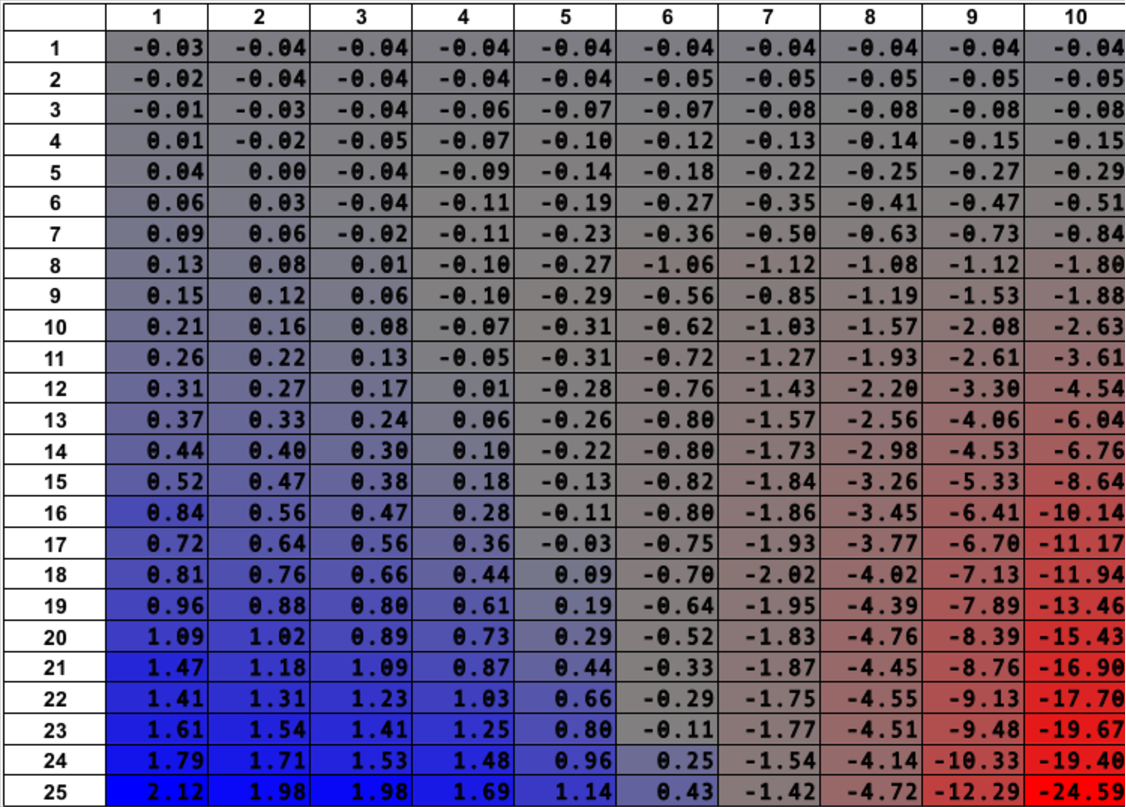
\includegraphics[
    width=\textwidth,
]{report_colors_cropped.pdf}
\end{figure}

For formulas given in DNF, the semantic algorithm is faster for formulas of any
	length,
	and the syntactic algorithm reaches Python's default maximum
	recursion depth 
        of $1000$ beginning at $3$ propositions.

The run time of the syntactic algorithm is agnostic to the number of unique
	propositions
        in the given formula since uniqueness of a proposition is primarily
        semantic notion.
The semantic algorithm is less concerned with the syntactic
        structure of the given formula since this has less bearing on the
        construction of a truth table.
The relative strengths of the two algorithms highlights two distinct ways that
        a propositional formula can be complex.

\subsection{Resolution}
Resolution is a proof method commonly used in automated theorem pr overs.

\subsubsection{Clausal Form}
Before implementing resolution, it is useful to have another way to
   represent propositional formulas.
We shall refer to a list of literals as a \emph{clause}.
A clause is satisfied if any of its literals are satisfied.
Thus a non-empty clause is equivalent to a disjunction of its members.
Note that an empty clause is unsatisfiable.
We shall say that a list of clauses is satisfied if all of clauses in the 
   list are satisfied.
Clearly a list of clauses containing an empty clause is unsatisfiable.
A list of non-empty clauses is equivalent to a formula in CNF.

We define the following utility function for converting a formula in CNF to
   a list of clauses (i.e., a list of lists of literals).
\begin{code}
def fml_to_clauses(f):
    if atom(f) or f[0] == 'not':
        return [[f]]
    if f[0] == 'or': 
        return [f[1]]
    if f[0] == 'and':
        return [fml_to_clauses(x)[0] for x in f[1]]
\end{code}


\subsubsection{The Resolution Rule}
The rule at the core of resolution is as follows:
Given two clauses:
\begin{align*}
A &= [a_1,...,a_{i-1}, p, a_{i},...,a_n]\text{ and }\\
B &= [b_1,...,b_{j-1},\lnot p, b_{j}, ..., b_m]
\end{align*}
such that each $a_i$ and $b_i$ are literals and $p$ is an atomic formula,
if $A$ and $B$ are both satisfied, then so 
   is $C = [a_1,..., a_n, b_1..., b_m]$.
Two clauses of the form $A$ and $B$ are call \emph{resolvable}.
We apply the resolution rule to a list of clauses by removing two resolvable
   clauses and replacing them with the result of resolving them.
Repeated application of the resolution rule will result in a list of clauses
   that are pairwise unresolvable.
If $[A_1,...,A_n]$ is a non-empty list of unresolvable clauses, it is easy 
   to see that it is satisfiable, since we may simply choose one literal 
   from each clause to make true, and doing so won't preclude the 
   satisfiability of any of the other clauses.
If any of the clauses is empty then the list is contradictory.
This is natural since the resolution rule can only give an
   empty clause is by resolving two contradictory singleton clauses:
\[
\big[A_1,..., A_{i-1}, [p], [\lnot p], A_i,..., A_n\big] \overset{resolve}\implies
\big[A_1,..., A_{i-1}, [\ ], A_i,..., A_n\big]
\]
Clearly once an empty clause produced, there is no need to resolve further;
   the list is unsatisfiable.

\subsubsection{Implementation}

The deduction theorem for propositional logic says that a sentence $\psi$
   follows from a finite list of sentences $\phi_1,...,\phi_n$ if and only
   if the implication formed by the conjunction of the $\phi_i$'s and $\psi$
   is a tautology:
\[
\phi_1,...,\phi_n\models\psi \iff \models\phi_1\land,...,\land\phi_n
   \rightarrow\psi
\]

A sentence is a tautology if and only if its negation is a contradiction.
The resolution rule can tell us whether a list of clauses is a contradiction.
Thus the problem of checking if $\phi_1,...,\phi_n\models\psi$ is reduced
   to checking whether or not a single sentence is contradictory.

\begin{code}
def resolve(f):
    return resolve_do(fml_to_clauses(cnf(('not', f))))
\end{code}

First we define a function that, given a list of clauses, searches for two
   that are resolvable and returns a triple containing the two clauses
   and the literal that makes them resolvable.

\begin{code}
def resolve_resolvable(clauses):
    for c1 in clauses:
        for lit in c1:
            if atom(lit):
                for c2 in clauses:
                    if c2 is c1:
                        continue
                    if ('not', lit) in c2:
                        return (lit, c1, c2)
\end{code}
If no resolvable clauses are found, the function will return \texttt{None}
   (Python's default return value).

Now we are ready to define the resolution algorithm:

\begin{code}
def resolve_do(clauses):

    res = resolve_resolvable(clauses)
    if not res:
        # No resolvable clauses were found.
        return False
    lit, c1, c2 = res

    # Apply the resolution rule.
    clauses.remove(c1)
    c1.remove(lit)
    clauses.remove(c2)
    c2.remove(('not',lit))
    clauses.append(c1 + c2)

    if [] in clauses:
        # The list of clauses is unsatisfiable.
        return True

    return resolve_do(clauses)
\end{code}

\subsection{Semantic Tableaux}

The semantic tableaux procedure is closely related to disjunctive normal form
(DNF). Analogous to CNF, a formula is in DNF if it is a disjunction of
subformulas, each which either is a literal or a conjunction of literals. As a
special case, a DNF formula may consist of only a single disjunct that is
either a literal or a conjunction of literals. We have implemented a syntactic
DNF algorithm that is symmetric to our implementation of the syntactic CNF
algorithm. Because of this symmetry, we omit the DNF implementation here.

To prove a formula $\phi$, the semantic tableaux procedure begins by taking
$\lnot\phi$ and then repeatedly applying so-called expansion rules to it. These
expansion rules expand $\lnot\phi$ into a tableau or tree with the following
properties. Each node is labelled by a subformula of $\lnot\phi$. Each branch
represents the conjunction of its nodes, while the tree itself represents the
disjunction of its branches. If the expansion is completed, the tree represents
a DNF formula equivalent to $\lnot\phi$.

The expansion rules work as follows. Given a tree, take a branch and a formula
$\psi$ on that branch. Then one of the following rules are applied.

\begin{itemize}
\item
If $\psi$ is of the form $\lnot\lnot\chi$, then add $\chi$ as a new node to the
branch.

\item
If $\psi$ is an alpha (i.e. conjunctive) formula, then add each conjunct of
$\psi$ as a new node to the branch.

\item
If $\psi$ is a beta (i.e. disjunctive) formula, then add each disjunct as a
new child to the last node of the branch.
\end{itemize}

We say that a branch is closed if it contains both a formula and its negation.
A tableau is closed if all of its branches are closed. Thus $\phi$ is proved if
the tableau for $\lnot\phi$ is closed.

\subsubsection{A Simple Semantic Tableaux Implementation}

The approach outlined above suggests a very simple semantic tableaux
implementation. We first call the \texttt{dnf()} function to transform the
formula into DNF. This will provide us with a finished tableau. We then only
have to check if all branches are closed.

\begin{code}
def tableau_dnf(f):
    return tableau_dnf_do(dnf(('not', f)))

def tableau_dnf_do(f):
    if literal(f):
        return False
    if f[0] == 'and':
        return any(atom(g) and ('not', g) in f[1] for g in f[1])
    else:
        return all(tableau_dnf_do(g) for g in f[1])
\end{code}

The drawback of this approach is that it requires the DNF transformation to be
completed before we can check for closure. It would be much more efficient if
we perform closure tests at earlier stages in the DNF transformation. This is
what we will look at now.

\subsubsection{A Better Tableaux Implementation}

Instead of using the \texttt{dnf()} function, we perform the expansion rules
described above. But before applying an expansion rule on a branch, we check if
the branch is closed. If it is, no further expansion of the branch is
necessary. We use the following function to check whether a branch is closed.

\begin{code}
def tableau_closed(branch):
    negations = [f for f in branch if f[0] == 'not']
    for f in negations:
        if f[1] in branch:
            return True
    return False
\end{code}

Now, the expansion rules are applied recursively by the following function. It
takes a single branch as argument, applies one expansion rule to a formula on
the branch and then calls itself with the resulting branch. If the expansion
rule results in multiple branches, it calls itself separately for each branch.

\begin{code}
def tableau_do(branch):
    if tableau_closed(branch):
        return True

    # Handle double negations and alpha formulas.
    for f in branch:
        if f[0] == 'not' and f[1][0] == 'not':
            return tableau_do([g for g in branch if g != f] + [f[1][1]])
        if f[0] == 'and':
            return tableau_do([g for g in branch if g != f] + f[1])
        if (f[0] == 'not' and f[1][0] == 'or'):
            return tableau_do([g for g in branch if g != f] +
                [('not', g) for g in f[1][1]])
        if (f[0] == 'not' and f[1][0] == 'arrow'):
            return tableau_do([g for g in branch if g != f] +
                [f[1][1], ('not', f[1][2])])

    # Handle beta formulas.
    for f in branch:
        if f[0] == 'or':
            return all(tableau_do([h for h in branch if h != f] + [g])
                for g in f[1])
        if f[0] == 'not' and f[1][0] == 'and':
            return all(tableau_do([h for h in branch if h != f] + [('not', g)])
                for g in f[1][1])
        if f[0] == 'arrow':
            return (tableau_do([g for g in branch if g != f] + [('not', f[1])])
                and tableau_do([g for g in branch if g != f] + [f[2]]))

    return False
\end{code}

Finally, the tableaux procedure is initiated by negating the formula to be
proved, putting it on a branch by itself and passing it to
\texttt{tableau\_do()}:

\begin{code}
def tableau(f):
    return tableau_do([('not', f)])
\end{code}

\section{Predicate Methods}

\subsection{Formula Representation}
% TODO Bill

\subsection{Unification}
% TODO Tim

\subsection{Skolemization}
% TODO Bill

\subsection{Tableaux}
% TODO Later


\end{document}
